% !TeX root = report_example.tex
\newcommand*{\MyHeaderPath}{.}% This path definition is also passed to inside the header files.
\newcommand*{\PathToAssets}{../assets}%
\newcommand*{\PathToOutput}{../output/}%
% \newcommand*{\PathToBibFile}{bibliography.bib}%
\documentclass{article}

% Language setting
% Replace `english' with e.g. `spanish' to change the document language
\usepackage[english]{babel}

% Set page size and margins
% Replace `letterpaper' with `a4paper' for UK/EU standard size
\usepackage[letterpaper,top=2cm,bottom=2cm,left=3cm,right=3cm,marginparwidth=1.75cm]{geometry}

% Useful packages
\usepackage{amsmath}
\usepackage{graphicx}
\usepackage[colorlinks=true, allcolors=blue]{hyperref}


\title{Replication of Nozawa, Yoshio's “What Drives the Cross‐Section of Credit Spreads?: A Variance Decomposition Approach.”}
\author{Julia Klauss, Joy Wu, Mengdi Hao, Yu-Ting Weng}

\begin{document}
\maketitle

\section{Introduction}

In this project, we replicate data and tables from Nozawa, Yoshio's “What Drives the Cross‐Section of Credit Spreads?: A Variance Decomposition Approach." In addition, we reproduce the data and tables with updated numbers until 2023/12/31. We replicate the corporate bond columns from the monthly test assets from He, Kelly, and Manela (2017). 

\section{ Data Collection and Preprossessing}

\subsection{Data Collection}

The panel data for corporate bond prices is constructed from three primary databases: Lehman Brothers Fixed Income Database, Mergent FISD/NAIC Database, and TRACE. The priority order for overlapping data is Lehman Brothers, TRACE, and Mergent FISD/NAIC. Lehman Brothers database covers from 1973/01 to 1998/03 and TRACE database covers from 2022/07 to 2023/12. The time gap between these two databases is filled by Mergent FISD/NAIC database.

Besides the above data sources on corporate bonds, the replication also involves using risk-free rate as the columns represent excess returns, which is calculated by corporate bond return minus a matching risk-free rate. Constant-maturity treasury yields are collected, according to Nozawa (2017), to calculate maturity-matching risk-free rate. There are 11 different maturities in the original treasury yields data: 1-month, 3-month, 6-month, 1-year, 2-year, 3-year, 5-year, 7-year, 10-year, 20-year, and 30-year. To find a matching risk-free rate for corporate bonds with different time-to-maturity, we conducted a cubic splines interpolation method to interpolate the original treasury yields. This interpolation process was done for every month during 1953/04 and 2024/01. The interpolation step is set to one month as our data frequency is monthly.After interpolation, we have monthly treasury yields from 1953/04 to 2024/01 for maturities from 1-month to 360-month.

\subsection{Data Prepossessing}

The merging process involves combining Lehman Brothers and TRACE data, and filling missing dates with Mergent FISD/NAIC.  As we utilize the WRDS Bond Return database, it's crucial to note that this source inherently includes monthly bond returns that account for defaults. We do not rely on Moody's Default Risk Service for complementing prices upon default. The dataset undergoes filtering to remove bonds with floating rates and non-callable options. Matching with synthetic Treasury bonds is performed to calculate excess returns and credit spreads. 

Data cleaning includes removing bonds with prices higher than matching Treasury bond prices and handling return observations showing significant bouncebacks. The final dataset is sorted into 10 columns based on yield spreads, each representing a U.S. corporate bond portfolio. This comprehensive process ensures a robust dataset for empirical analysis. 

\subsection{Difficulties}

Difficulties arose during our replication efforts, specifically in the treasury matching section. In the initial step, we conducted cubic spline interpolation to derive the Treasury yield curve and subsequently constructed Treasury zero-coupon yield curves through the bootstraping method. This provided results covering the period from July 1, 1992, to January 1, 2024, which were stored in the file "Treasury Zero Coupon Rate.csv". However, due to NaN values in the "Monthly Treasury Yield.csv" dataset, we couldn't extend this process to the earlier period from January 1, 1973, to June 1, 1992. 

Additionally, we faced challenges in removing bonds with floating rates and with option features, other than callable bonds, as described in the data processing section of the Nozawa paper. We had difficulty including the necessary variables to filter those bonds when loading the Mergent data while still maintaining an automated data retrieval process. Due to this, our replicated data still includes the bonds with floating rates and with option features. 

\section{ Unit Testing}

To compare the data we replicate to the given sample dataframe (He, Kelly, and Manela (2017)),  we select specific columns for testing, focusing on a randomly chosen short period from September 2003 to December 2003. The test checks if the replicated data is similar to the sample data within a tolerance of 5\%. Additionally, we conduct a test on the mean values for a more extended period, covering the years 1975 to 1997. This test employs a smaller tolerance of 4\% for mean comparison. We set these tolerance levels due to the presence of outliers in the data. The unit test ensures that the replicated data aligns with the expected data within the specified tolerance levels.

To visualize the similarity, we employ another method by graphing the data into a comparison line plot (Figure 1). It illustrates how the replicated data aligns with the sample dataframe over most of the selected time periods.

\begin{figure} [h]
    \centering
    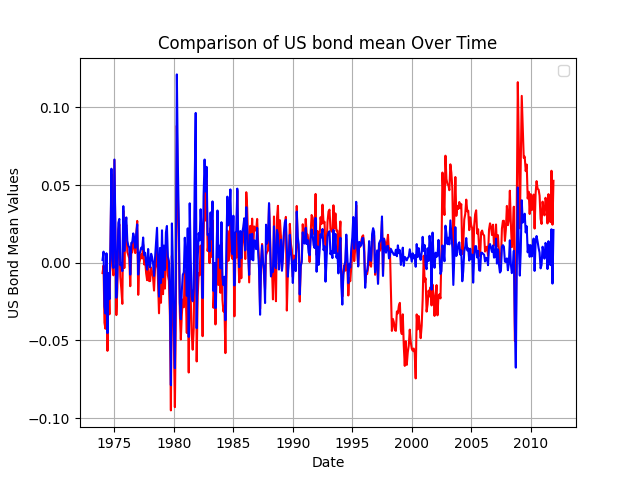
\includegraphics[width=0.75\linewidth]{output/comparison_lineplot.png}
    \caption{Comparison Line Plot}
    \label{fig:comparison plot}
\end{figure}
\clearpage  % Start a new page

\section{ Summary Statistic Tables}
To compare bond portfolios across dataframes, three summary statistics tables were generated. Tables 1 and 2 correspond to the He, Kelly, and Manela (2017) dataframe. Tables 3 and 4 represent data replicated from 1973 to 2012, matching the paper's period. Tables 5 and 6 showcase data replicated from 1973 and updated to 2023.  
\\
The breakdown of key statistical measures for the US Bond Portfolios 11-20 is detailed as follows: 

\subsection{He, Kelly, and Manela (2017)}
\begin{table}[h] 
\centering 
   \caption{Summary Statistics of Sample Dataframe}
   \begin{tabular}{lrrrrr}
\toprule
group &  US Bonds 11  &  US Bonds 12  &  US Bonds 13  &  US Bonds 14  &  US Bonds 15  \\
\midrule
count  &  456.000000  &  456.000000  &  456.000000  &  456.000000  &  456.000000  \\
mean  &  0.005923  &  0.006518  &  0.006743  &  0.006581  &  0.007048  \\
std  &  0.018431  &  0.019738  &  0.020000  &  0.020199  &  0.020059  \\
min  &  -0.078800  &  -0.076400  &  -0.078300  &  -0.078600  &  -0.081800  \\
25\%  &  -0.002600  &  -0.003225  &  -0.003125  &  -0.002800  &  -0.002525  \\
50\%  &  0.006200  &  0.006400  &  0.006300  &  0.006700  &  0.006900  \\
75\%  &  0.014125  &  0.015925  &  0.016325  &  0.016625  &  0.016800  \\
max  &  0.127400  &  0.124300  &  0.132600  &  0.120700  &  0.126800  \\
\bottomrule
\end{tabular}
\end{table}

\begin{table}[h] 
\centering 
   \caption{Summary Statistics of Sample Dataframe}
   \begin{tabular}{lrrrrr}
\toprule
group &  US Bonds 16  &  US Bonds 17  &  US Bonds 18  &  US Bonds 19  &  US Bonds 20 \\ \\
\midrule
count  &  456.000000  &  456.000000  &  456.000000  &  456.000000  &  456.000000 \\ \\
mean  &  0.007016  &  0.007262  &  0.007460  &  0.007438  &  0.010098 \\ \\
std  &  0.019479  &  0.018882  &  0.018618  &  0.018568  &  0.023779 \\ \\
min  &  -0.080200  &  -0.081700  &  -0.083500  &  -0.087200  &  -0.102100 \\ \\
25\%  &  -0.002200  &  -0.000725  &  -0.000125  &  0.000575  &  0.000300 \\ \\
50\%  &  0.007250  &  0.007600  &  0.007900  &  0.007950  &  0.010000 \\ \\
75\%  &  0.015900  &  0.015425  &  0.015125  &  0.015000  &  0.020225 \\ \\
max  &  0.129300  &  0.125700  &  0.128800  &  0.110300  &  0.148300 \\ \\
\bottomrule
\end{tabular}
\end{table}


\subsection{Replicated Data from 1973 to 2012}
\begin{table}[h] 
\centering 
   \caption{Summary Statistics 1973-2012}
   \begin{tabular}{lrrrrr}
\toprule
group &  US Bonds 11  &  US Bonds 12  &  US Bonds 13  &  US Bonds 14  &  US Bonds 15  \\
\midrule
count  &  478.000000  &  478.000000  &  478.000000  &  478.000000  &  478.000000  \\
mean  &  0.002338  &  -0.004300  &  -0.002913  &  -0.000495  &  0.001687  \\
std  &  0.036965  &  0.029175  &  0.028949  &  0.029031  &  0.028787  \\
min  &  -0.093312  &  -0.098303  &  -0.098917  &  -0.097085  &  -0.098487  \\
25\%  &  -0.021043  &  -0.021642  &  -0.021749  &  -0.018586  &  -0.016675  \\
50\%  &  0.002808  &  -0.004252  &  -0.002728  &  0.000639  &  0.003401  \\
75\%  &  0.023688  &  0.014117  &  0.016401  &  0.019164  &  0.020761  \\
max  &  0.113758  &  0.118031  &  0.119924  &  0.125013  &  0.111733  \\
\bottomrule
\end{tabular}
\end{table}
\clearpage  % Start a new page
\begin{table}[h]
\centering 
   \caption{Summary Statistics 1973-2023}
   \begin{tabular}{lrrrrr}
\toprule
group &  US Bonds 16  &  US Bonds 17  &  US Bonds 18  &  US Bonds 19  &  US Bonds 20 \\ 
\midrule
count  &  478.000000  &  478.000000  &  478.000000  &  478.000000  &  478.000000 \\ 
mean  &  0.003786  &  0.006748  &  0.010782  &  0.016120  &  0.030652 \\ 
std  &  0.029212  &  0.029761  &  0.031267  &  0.035966  &  0.056445 \\ 
min  &  -0.095305  &  -0.093099  &  -0.094998  &  -0.165497  &  -0.309571 \\ 
25\%  &  -0.014572  &  -0.010091  &  -0.006654  &  -0.001684  &  0.008136 \\ 
50\%  &  0.006102  &  0.010040  &  0.014366  &  0.019809  &  0.032313 \\ 
75\%  &  0.021975  &  0.026171  &  0.029580  &  0.034412  &  0.056826 \\ 
max  &  0.110175  &  0.110108  &  0.125269  &  0.199137  &  0.310583 \\ 
\bottomrule
\end{tabular}
\end{table}


\subsection{Replicated Data from 1973, Updated to 2023 }
\begin{table}[h]
\centering
   \caption{Summary Statistics 1973-2023}
   \begin{tabular}{lrrrrr}
\toprule
group &  US Bonds 11  &  US Bonds 12  &  US Bonds 13  &  US Bonds 14  &  US Bonds 15  \\
\midrule
count  &  610.000000  &  610.000000  &  610.000000  &  610.000000  &  610.000000  \\
mean  &  0.004173  &  -0.000340  &  0.001049  &  0.003120  &  0.004884  \\
std  &  0.033956  &  0.027675  &  0.027716  &  0.027997  &  0.028021  \\
min  &  -0.093312  &  -0.098303  &  -0.098917  &  -0.097085  &  -0.098487  \\
25\%  &  -0.015724  &  -0.018066  &  -0.018298  &  -0.015176  &  -0.013293  \\
50\%  &  0.005464  &  0.002730  &  0.003987  &  0.005681  &  0.007320  \\
75\%  &  0.023491  &  0.019285  &  0.021357  &  0.022354  &  0.023688  \\
max  &  0.113758  &  0.118031  &  0.119924  &  0.125013  &  0.111733  \\
\bottomrule
\end{tabular}
\end{table}
\begin{table}[h]
\centering
   \caption{Summary Statistics 1973-2023}
   \begin{tabular}{lrrrrr}
\toprule
group &  US Bonds 16  &  US Bonds 17  &  US Bonds 18  &  US Bonds 19  &  US Bonds 20 \\ 
\midrule
count  &  610.000000  &  610.000000  &  610.000000  &  610.000000  &  610.000000 \\ 
mean  &  0.006722  &  0.009466  &  0.013479  &  0.018892  &  0.033779 \\ 
std  &  0.028509  &  0.029099  &  0.030381  &  0.034842  &  0.055932 \\ 
min  &  -0.095305  &  -0.093099  &  -0.094998  &  -0.165497  &  -0.327369 \\ 
25\%  &  -0.011864  &  -0.007385  &  -0.003567  &  0.002961  &  0.009479 \\ 
50\%  &  0.009574  &  0.013648  &  0.017376  &  0.022509  &  0.036811 \\ 
75\%  &  0.024532  &  0.027742  &  0.031263  &  0.037153  &  0.058832 \\ 
max  &  0.110175  &  0.110108  &  0.125269  &  0.199137  &  0.310583 \\ 
\bottomrule
\end{tabular}
\end{table}

\section{ Comparison and Conclusion}
In comparing the summary statistics of US bond portfolios 11-20 derived from our replicated data for the period 1973-2012 with the sample data from the paper, several observations can be made. Despite the omission of some preprocessing steps in our data replication process, the mean returns of each portfolio in our dataset closely resemble those in the paper. The majority of portfolios exhibit minimal differences, with variances typically within 0.01.
\\\\ 
However, notable distinctions emerge for portfolios with larger yield spreads. These portfolios demonstrate more significant differences, suggesting that the replication accuracy may be influenced by the specific characteristics of the bond portfolios. The impact of omitted preprocessing steps on these particular portfolios warrants further investigation. 
\\\\ 
While our replication aligns well with the mean returns of most portfolios, the observed differences emphasize the importance of meticulous data preprocessing steps, especially when dealing with portfolios exhibiting greater variability in yields. Future work could focus on refining the replication process to address these differences and enhance the overall accuracy of the replicated dataset. 

\bibliographystyle{alpha}
\bibliography{sample}
\\\\
[1] WRDS Corporate Bond Database: Data Overview and Construction Manual, WRDS Research April 2017,\\
(https://wrds-www.wharton.upenn.edu/documents/248/WRDS_Corporate_Bond_Database_Manual.pdf.)
\\\\
[2] Arthur Warga, Lehman Brothers Fixed Income Database, Jan 1973 - Dec 1997. 2000, \\(http://www.columbia.edu/acis/eds/holdings/1021/. )
\\\\
[3] Gwangheon Hong, & Warga, A. (2000). An Empirical Study of Bond Market Transactions. \\Financial Analysts Journal, 56(2), 32-46.
\\\\
[4] Nianyun (Kelly) Cai, Jean Helwege, Arthur Warga, Underpricing in the Corporate Bond Market, \\The Review of Financial Studies, Volume 20, Issue 6, November 2007, Pages 2021-2046, \\(https://doi.org/10.1093/rfs/hhm048)
\\\\
[5] Mergent FISD Transactions (Fisd_naic). 28 July 2023,\\ (https://wrds-www.wharton.upenn.edu/data-dictionary/fisd_naic/. )
\\\\
[6] US  Treasury Database Guide For SAS, ASCII, EXCEL \& R. CRSP Center For Research in Security Prices, LLC, \\(https://drive.google.com/file/d/1joqukSE4P4noGmPH8fcbg5fGURtJfFIL/view. )
\\\\
[7] He, Zhiguo, et al. Intermediary Asset Pricing: \\New Evidence from Many Asset Classes. Journal of Financial Economics, 12 Aug. 2017. 
\\\\
[8] NOZAWA, YOSHIO. What Drives the Cross-Section of Credit Spreads?: A   Variance Decomposition Approach. \\The Journal of Finance, Oct. 2017, DOI: 10.1111/jofi.12524. 
\end{document}
